\section{Dados do sensor laser}
Essa Seção explica o formato dos dados brutos do sensor LiDAR, e como eles 
são processados e transformados nos dados utilizados pelo modelo de medida 
descrito na Seção \ref{sec:slam-measurement} (\nameref{sec:slam-measurement}).

\subsection{Dados brutos}
Os dados brutos do sensor LiDAR utilizado, consistem numa sequência de 
distâncias $\{r^0, r^1, \dots, r^N\}$. Esses valores são gerados pela reflexão de feixes de laser, emitidos pelo sensor, nas superfícies 
presentes no ambiente. Os feixes são disparados de maneira sequencial no 
sentido anti-horário a partir do eixo $x$ do sistema de coordenadas do sensor. 
Além disso, o sensor também fornece as posições angulares $\theta_0$ 
do primeiro e $\theta_N$ do último feixe, e o incremento na posição angular $\Delta \theta$ entre o feixe $k$ e o feixe $k+1$.

A Figura \ref{fig:sensor-raw-data} apresenta os dados brutos obtidos em uma 
leitura feita no ambiente mostrado na Figura \ref{fig:environment}.
\begin{figure}[h]
  \centering
  \begin{subfigure}{0.6\textwidth}
    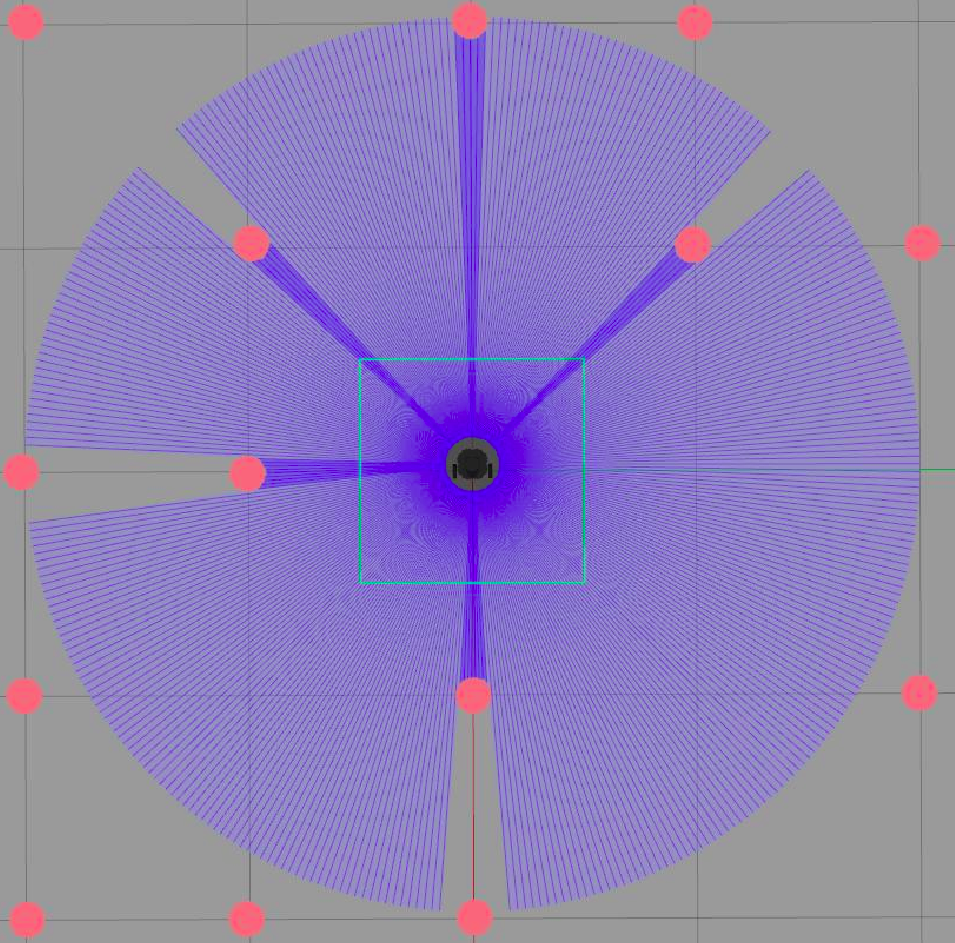
\includegraphics[width=\textwidth, angle=90]{figs/sensor-simulation-view.png}
    \caption{Representação dos feixes laser (em azul) emitidos pelo sensor LiDAR com 
    alcance máximo de 2 metros. Os círculos em rosa representam as landmarks.}
    \label{fig:laser-beams-visualization}
  \end{subfigure}
  \begin{subfigure}{0.8\textwidth}
    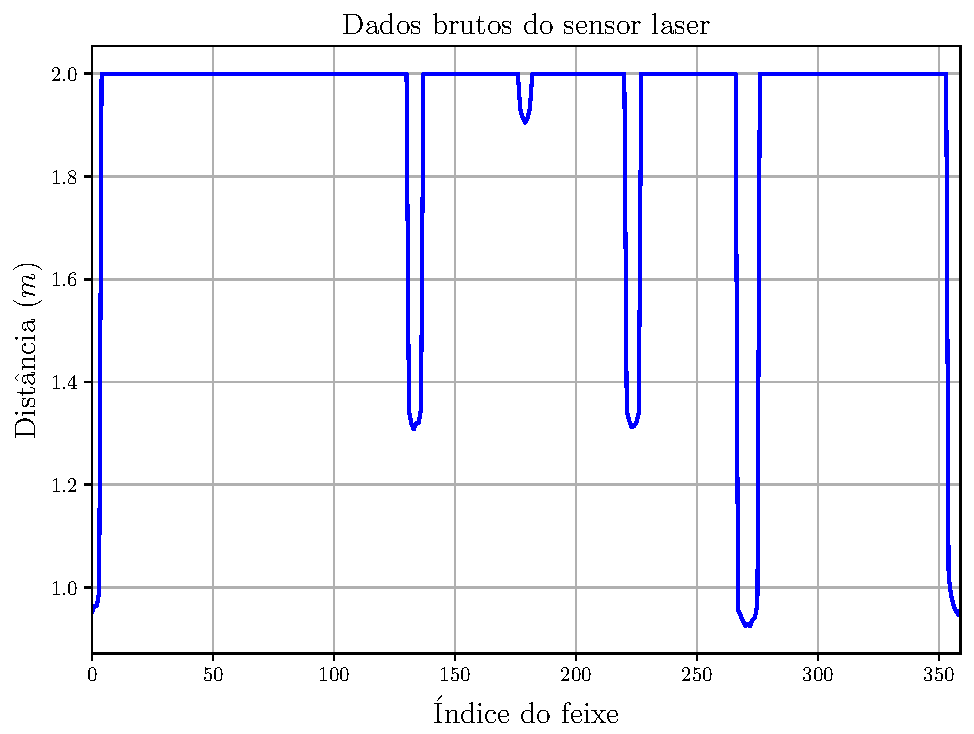
\includegraphics[width=\textwidth]{figs/raw_sensor_data.pdf}
    \caption{Interpolação linear das distâncias lidas pelo sensor.}
    \label{fig:sensor-raw-data}
  \end{subfigure}
  \caption{Visualização dos feixes laser emitidos pelo sensor LiDAR e a 
  respectiva leitura gerada.}
  \label{fig:sensor-visualization-and-reading}
\end{figure}

\subsection{Processamento de dados}
Para transformar o dado bruto, a sequência de distâncias na Figura 
\ref{fig:sensor-raw-data}, nas medidas consumidas pelo modelo de medida 
descrito na Seção \emph{\nameref{sec:slam-measurement}}, é proposto um 
\textit{pipeline} de processamento de dados, Figura \ref{fig:lidar-data-processing-pipeline},cujo último estágio é o 
algoritmo de estimação de círculos a partir de pontos em coordenadas 
cartesianas \cite[p.~903]{al2009error}.

\begin{figure}[h]
  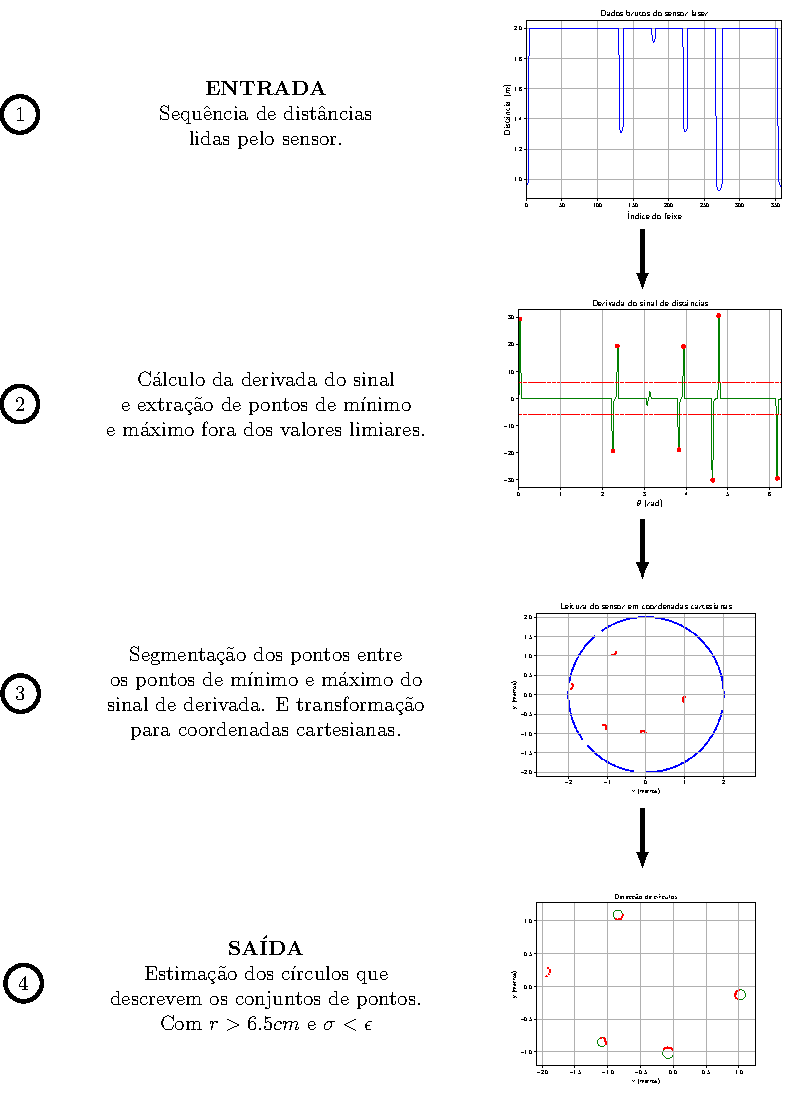
\includegraphics[width=\textwidth]{figs/data_processing_pipeline.pdf}
  \caption{Sequência de passos para processar os dados brutos do sensor LiDAR e
  transforma-los em dados úteis para o modelo de medida utilizado.}
  \label{fig:lidar-data-processing-pipeline}
\end{figure}

Para começar, é necessário extrair os pontos que correspondem à reflexões nas 
superfícies dos cilindros presentes no ambiente. Para isso, observa-se que há uma variação brusca nas distâncias lidas pelo sensor quando os feixes são 
refletidos pelas superfícies dos cilindros. Ao analisar a derivada do sinal, 
representada na Figura \ref{fig:sensor-derivative}, podemos notar que o intervalo de medidas 
correspondente à reflexões dos cilindros se encontram entre uma variação 
positiva seguida rapidamente de uma variação negativa na curva da derivada.
\begin{figure}[h]
  \centering
  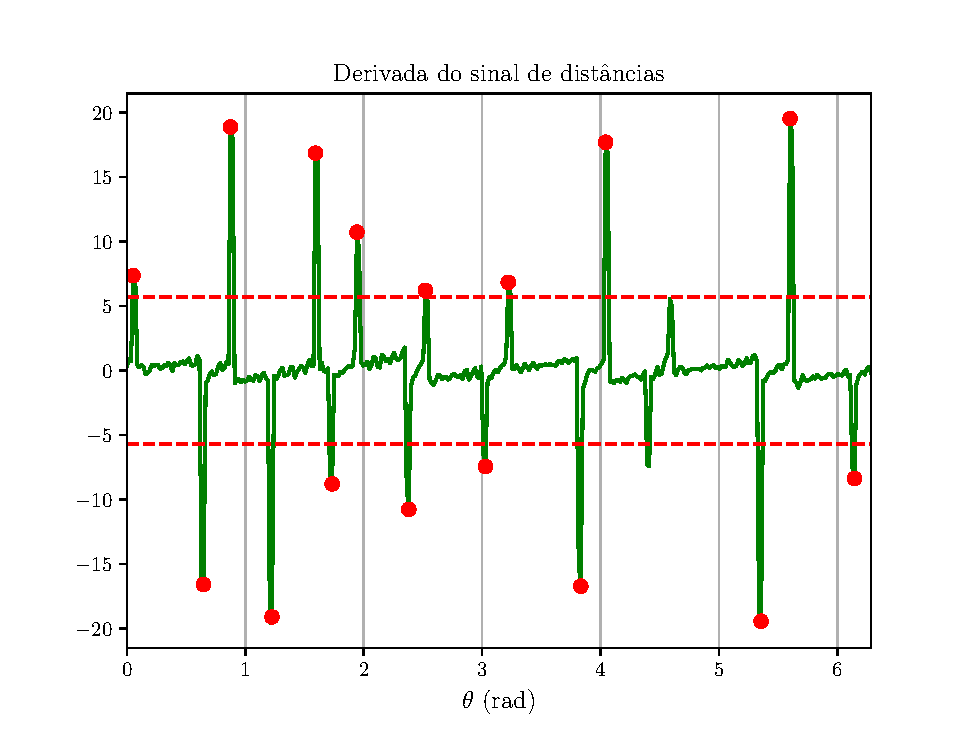
\includegraphics[width=.6\textwidth]{figs/signal_derivative.pdf}
  \caption{Derivada central da sequência de distâncias representadas na Figura \ref{fig:sensor-raw-data}. As linhas pontilhadas em vermelho 
  representam os limiares a partir dos quais os picos são interpretados 
  como início ou fim da superfície de um cilindro. Os picos destacados 
  em vermelho ultrapassam as valores limiares.}
  \label{fig:sensor-derivative}
\end{figure}

O próximo passo consiste em transformar o sinal para a representação em 
coordenadas cartesianas, e segmentar os conjuntos de pontos correspondentes aos intervalos entre picos e vales do sinal de derivada computado anteriormente, como é mostrado na Figura \ref{fig:sensor-data-cartesian}.
Então, cada um desses conjuntos é fornecido como entrada do Algoritmo 
\ref{alg:circle-fit} (listado no Anexo \ref{annex:circle-fit}), o resultado 
são círculos que melhor explicam esses conjuntos de pontos (Figura \ref{fig:detected-circles}), juntamente com o 
erro médio quadrático entre cada conjunto de pontos e seu círculo.
\begin{figure}[h]
  \centering
  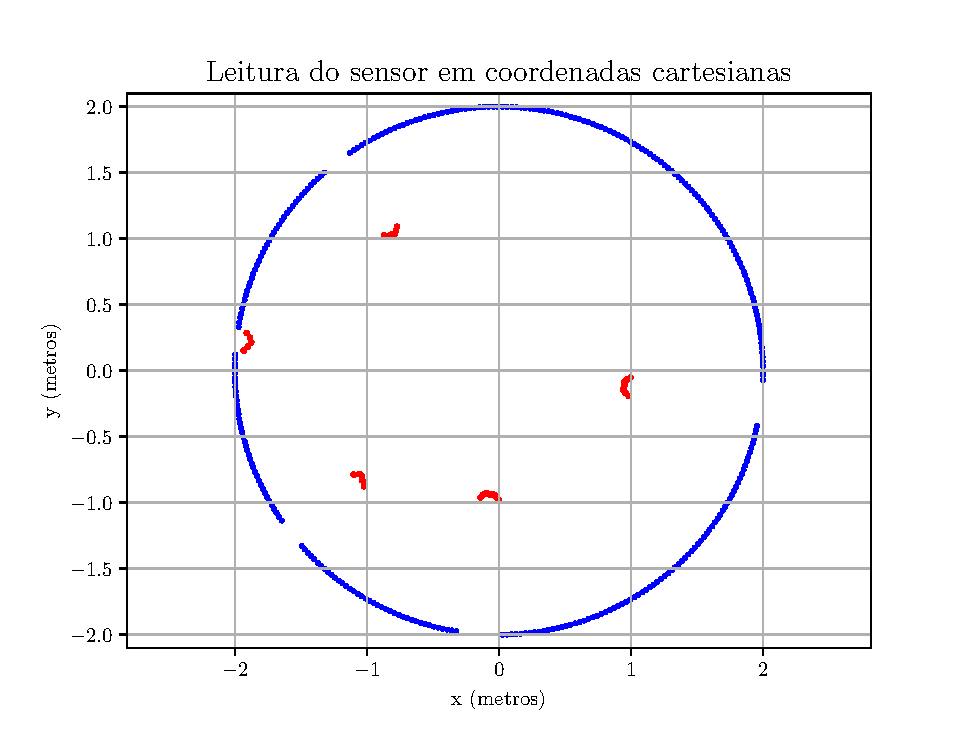
\includegraphics[width=.8\textwidth]{figs/sensor_data_cartesian.pdf}
  \caption{Representação da leitura do sensor LiDAR em coordenadas 
  cartesianas. Os pontos destacados em vermelho correspondem a reflexões 
  das superfícies das \textit{landmarks}.}
  \label{fig:sensor-data-cartesian}
\end{figure}

Por fim são considerados apenas os círculos cujo erro médio quadrático para 
seus pontos correspondentes é inferior a um limiar $\epsilon = 10^{-3}$ e 
cujo raio seja superior a 6cm. Essa última condição é especialmente útil no 
cenário multiagente, pois evita de que um robô confunda o sensor LiDAR (que 
fica montado no topo do robô, conforme visto na Figura \ref{fig:turtlebot-digital-twin}) do outro com uma \textit{landmark}.

\begin{figure}[h]
  \centering
  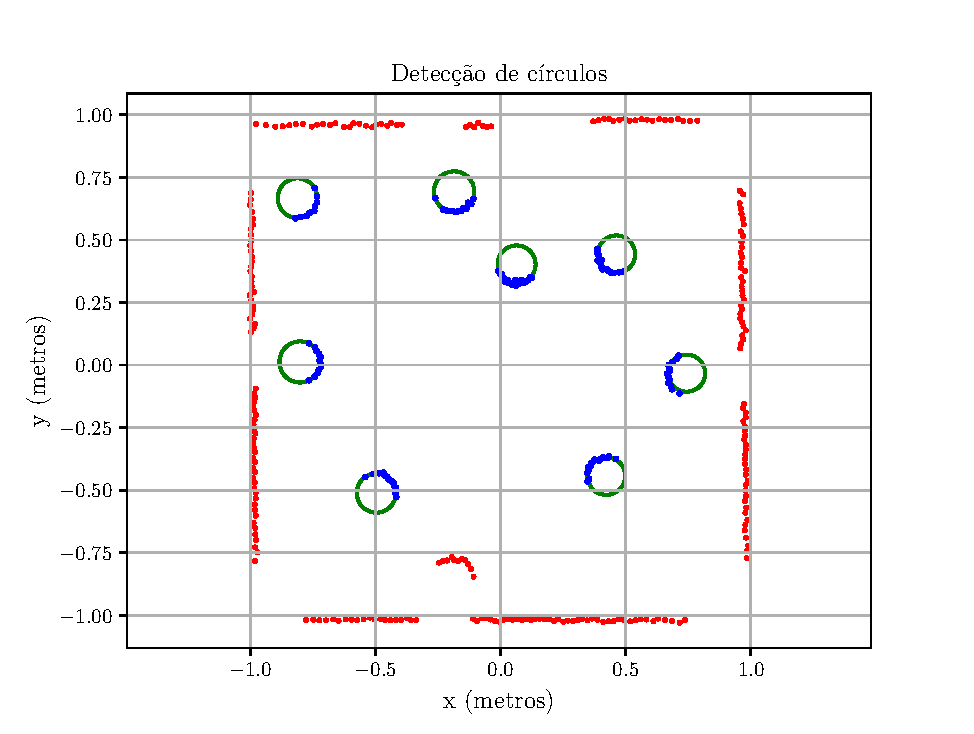
\includegraphics[width=.8\textwidth]{figs/circle_detection.pdf}
  \caption{Em vermelho, os conjuntos de pontos selecionados como pertencentes à superfícies das \textit{landmarks}. Em verde, os círculos 
  estimados para cada conjunto.}
  \label{fig:detected-circles}
\end{figure}

\section{Mapa em grade}
teste

\section{Exploração Autônoma}
teste
